\documentclass[12pt]{report}
\setlength{\textwidth}{6.5 in}
\setlength{\evensidemargin}{0 in}
\setlength{\oddsidemargin}{0 in}
\setlength{\textheight}{9.4 in }
\setlength{\topmargin}{-0.7 in}
\pagestyle{myheadings}
\markboth{\em EE264: Homework \#04}{\em EE264: Homework \#04}
\usepackage[pdftex]{graphicx} \usepackage{eso-pic}
\usepackage{amsmath}
\usepackage{amssymb}
\usepackage{graphicx}
\usepackage{ifthen}
\usepackage{tikz}
\usepackage{pgfplots}
\usepackage{array}  % for table column M
\usepackage{makecell} % to break line within a cell
\usepackage{verbatim}
\usepackage{epstopdf}
\usepackage{amsfonts}
\usepackage{xcolor}
\usepackage{subcaption}
\usepackage{pdfpages}
\usepackage{hyperref}
%\captionsetup{compatibility=false}
%\usepackage{dsfont}
\usepackage[absolute,overlay]{textpos}
\usetikzlibrary{calc, angles,quotes}
\usetikzlibrary{pgfplots.fillbetween, backgrounds}
\usetikzlibrary{positioning}
\usetikzlibrary{arrows}
\usetikzlibrary{pgfplots.groupplots}
\usetikzlibrary{arrows.meta}
\usetikzlibrary{plotmarks}
\usetikzlibrary{decorations.markings}

\DeclareGraphicsExtensions{.pdf,.eps,.png}

\DeclareMathOperator{\E}{\mathbb{E}} % expectation

\def\thickness{very thick}

\tikzset{
amark/.style 2 args={
	decoration={             
		markings, 
		mark=at position {0.5} with { 
			\arrow{stealth},
			\node[#2] {#1};
		}
	}, \thickness,
	postaction={decorate}
},
earlymark/.style 2 args={
	decoration={             
		markings, 
		mark=at position {0.25} with { 
			\arrow{stealth},
			\node[#2] {#1};
		}
	}, \thickness,
	postaction={decorate}
},
latemark/.style 2 args={
	decoration={             
		markings, 
		mark=at position {0.8} with { 
			\arrow{stealth},
			\node[#2] {#1};
		}
	}, \thickness,
	postaction={decorate}
},
zpath/.style={
	decoration={             
		markings, 
		mark=at position {0.5} with { 
			\arrow{stealth},
			\node[#1] {$z^{-1}$};
		}
	}, \thickness,
	postaction={decorate}
},
terminal/.style 2 args={draw,circle,inner sep=2pt,label={#1:#2}},
}


\newcommand\SimpleSys[4]{%
	\def\xin{#2}%
	\def\Hz{#3}%
	\def\yout{#4}
	\input{#1}%
}

\begin{document}
\thispagestyle{empty}
\begin{centering}
	{\large Stanford University}\\
	{\large EE 264: Digital Signal Processing}\\
	{\large Summer, 2017} \\
	\mbox{}\\
	{\large Homework \#04}\\
	\mbox{}\\
\end{centering}
\noindent Date assigned:  July 21, 2017 \hfill
Date due: July 30, 2017\\
\noindent \rule{6.5 in}{0.5pt}
%\mbox{}\\
\noindent {\bf Reading:}  This assignment covers primarily lectures 6 to 8, which correspond to chapters 5 and 6 of the textbook {\bf DTSP 3e}. \\
\noindent {\bf Homework submission:}  Please submit your solutions on Canvas. Create a single .pdf file containing all your analytical derivations, sketches, plots, and Matlab code (if applicable). \\
\noindent {\bf Extensions and late submissions:}  To ensure that we can release the solutions of this assignment in a timely manner for the midterm, we \underline{cannot} grant extensions or accept late submissions.

\noindent
\rule{6.5 in}{0.5pt}
\mbox{}\\

\noindent {\bf Problem 0: ($2\%$ extra points in final grade)} 

Fill out the mid-quarter teaching evaluation survey:
 \url{https://vptleval.stanford.edu/auth/evaluation.php?id=12580}
 
\mbox{}\\ 
\noindent {\bf Problem 1: (20 points)} 
A causal LTI system has the system function
\begin{equation}
H(z) = \frac{(1-e^{j\pi/3} z^{-1})(1-e^{-j\pi/3}z^{-1})(1+(1/0.85)z^{-1})}{(1-0.9e^{j\pi/3} z^{-1})(1-0.9e^{-j\pi/3}z^{-1})(1+0.85z^{-1})}
\end{equation}

\begin{description}
	\item{(a)} Plot the pole-zero diagram using Matlab's \texttt{zplane} function and indicate the region of convergence for the system function. 
	
	\textit{Hint:} Use the function \texttt{conv} to multiply out the denominator and numerator factors. The \texttt{conv} function is also used for the multiplication of polynomials.
	
	\item{(b)} Either plot or sketch the magnitude and phase responses of $H(e^{j\omega})$.
	
	\item{(c)} Either plot or sketch the group delay of $H(e^{j\omega})$. For the group delay you can use the Matlab function \texttt{grpdelay}. You may also numerically derivate the unwrapped phase to obtain the group delay.
	
	\item{(d)} State whether the following statements about $H(z)$ are true or false. Justify your answers. 
	\begin{enumerate}
		\item The system is stable
		\item The impulse response of that system approaches a non-zero value as $n\to\infty$.
		\item Since the system function has a pole at angle $\pi/3$ the magnitude of the frequency response has a peak at approximately $\omega=\pi/3$.
		\item The system is a minimum phase system.
		\item The system has a causal and stable inverse.
	\end{enumerate}
\end{description}

\noindent {\bf Problem 2: (25 points)} 

$H(z)$ is the system function for a \underline{stable} and \underline{causal} LTI system and is given by:
\begin{equation}
H(z) = \frac{(1-9z^{-2})(1+(1/3)z^{-1})}{(1-(1/3)z^{-1})}
\end{equation}

\begin{description}
	\item[(a)] $H(z)$ can be represented as a cascade of a minimum-phase system $H_{min}(z)$ and a unit-gain all-pass system $H_{ap}(z)$; i.e., $H(z) = H_{min}(z)H_{ap}(z)$. Determine a choice for $H_{min}(z)$ and $H_{ap}(z)$ and specify whether or not they are unique up to a scale factor.
	\item[(b)] Is the minimum-phase system, $H_{min}(z)$ in part (a) an FIR system? Explain.
	\item[(c)] For generalized linear phase FIR systems with \underline{real} coefficients, show that if $z = c$ is a zero, then $c^*, 1/c, 1/c^*$ must also be zeros. In words, zeros of generalized linear phase FIR systems appear in conjugate and conjugate reciprocal pairs.
	\item[(d)] Can $H(z)$ be represented as a cascade of a FIR generalized linear-phase system $H_{lin}(z)$ and an all-pass system $H_{ap2}(z)$; i.e., $H(z) = H_{lin}(z)H_{ap2}(z)$? If your answer is yes, determine $H_{lin}(z)$ and $H_{ap2}(z)$. If your answer is no, explain why such a representation does not exist.
\end{description}

\mbox{}\\ 
\noindent {\bf Problem 3: (25 points)} (adapted from several previous midterms)

Answer the following questions about the causal LTI systems having the pole-zero given in Figure~\ref{fig:pole-zero-diagram}.

In each case \underline{explain} why you chose the ones that you chose.

\begin{description}
	\item{(a) } Which systems are FIR systems? \\
	\hspace{10cm} (A)  \hspace{1cm}  (B)  \hspace{1cm}  (C) \hspace{1cm} (D) \hspace{1cm}  (E) \hspace{1cm} (F) \hspace{1cm} none \hspace{1cm}  all
	
	\item{(b) } Which systems are stable systems? \\
	\hspace{10cm} (A)  \hspace{1cm}  (B)  \hspace{1cm}  (C) \hspace{1cm} (D) \hspace{1cm}  (E) \hspace{1cm} (F) \hspace{1cm} none \hspace{1cm}  all
	
	\item{(c) } Which systems are \underline{probably}\footnotemark  all-pass systems, i.e., ${|H(e^{j\omega)}|}^2=$ constant for all $\omega$? \\
	\hspace{10cm} (A)  \hspace{1cm}  (B)  \hspace{1cm}  (C) \hspace{1cm} (D) \hspace{1cm}  (E) \hspace{1cm} (F) \hspace{1cm} none \hspace{1cm}  all
	
	\footnotetext{The word \underline{probably} is used because it is not possible to know the exact coordinates of the pole and zeros. However, you should make a favorable estimate of the locations when trying to match a property.}
	
	\item{(d) } Which systems are minimum-phase systems? \\
	\hspace{10cm} (A)  \hspace{1cm}  (B)  \hspace{1cm}  (C) \hspace{1cm} (D) \hspace{1cm}  (E) \hspace{1cm} (F) \hspace{1cm} none \hspace{1cm}  all
	
	\item{(e) } Which systems are \underline{probably} linear-phase systems? \\
	\hspace{10cm} (A)  \hspace{1cm}  (B)  \hspace{1cm}  (C) \hspace{1cm} (D) \hspace{1cm}  (E) \hspace{1cm} (F) \hspace{1cm} none \hspace{1cm}  all
	
	\item{(f) } Which systems have $H(e^{j\pi})=0$? \\
	\hspace{10cm} (A)  \hspace{1cm}  (B)  \hspace{1cm}  (C) \hspace{1cm} (D) \hspace{1cm}  (E) \hspace{1cm} (F) \hspace{1cm} none \hspace{1cm}  all
	
	\item{(g) } Which systems have \underline{lowpass} frequency response? \\
	\hspace{10cm} (A)  \hspace{1cm}  (B)  \hspace{1cm}  (C) \hspace{1cm} (D) \hspace{1cm}  (E) \hspace{1cm} (F) \hspace{1cm} none \hspace{1cm}  all
	
	\item{(h) } Which system has the shortest (least number of non-zero samples) impulse response? \\
	\hspace{10cm} (A)  \hspace{1cm}  (B)  \hspace{1cm}  (C) \hspace{1cm} (D) \hspace{1cm}  (E) \hspace{1cm} (F) \hspace{1cm} none \hspace{1cm}  all
	
	\item{(i) } Which systems have corresponding stable and causal inverse systems? \\
	\hspace{10cm} (A)  \hspace{1cm}  (B)  \hspace{1cm}  (C) \hspace{1cm} (D) \hspace{1cm}  (E) \hspace{1cm} (F) \hspace{1cm} none \hspace{1cm}  all
	
	\item{(j) } For the system labeled \textbf{C}, write the system function $H(z)$ as the product of a minimum phase function and an all-pass function. Assume that all the poles have radius 0.8, and the zeros outside the unit circle have radius 1.1.
\end{description}

\begin{figure}[h!]
	\centering
	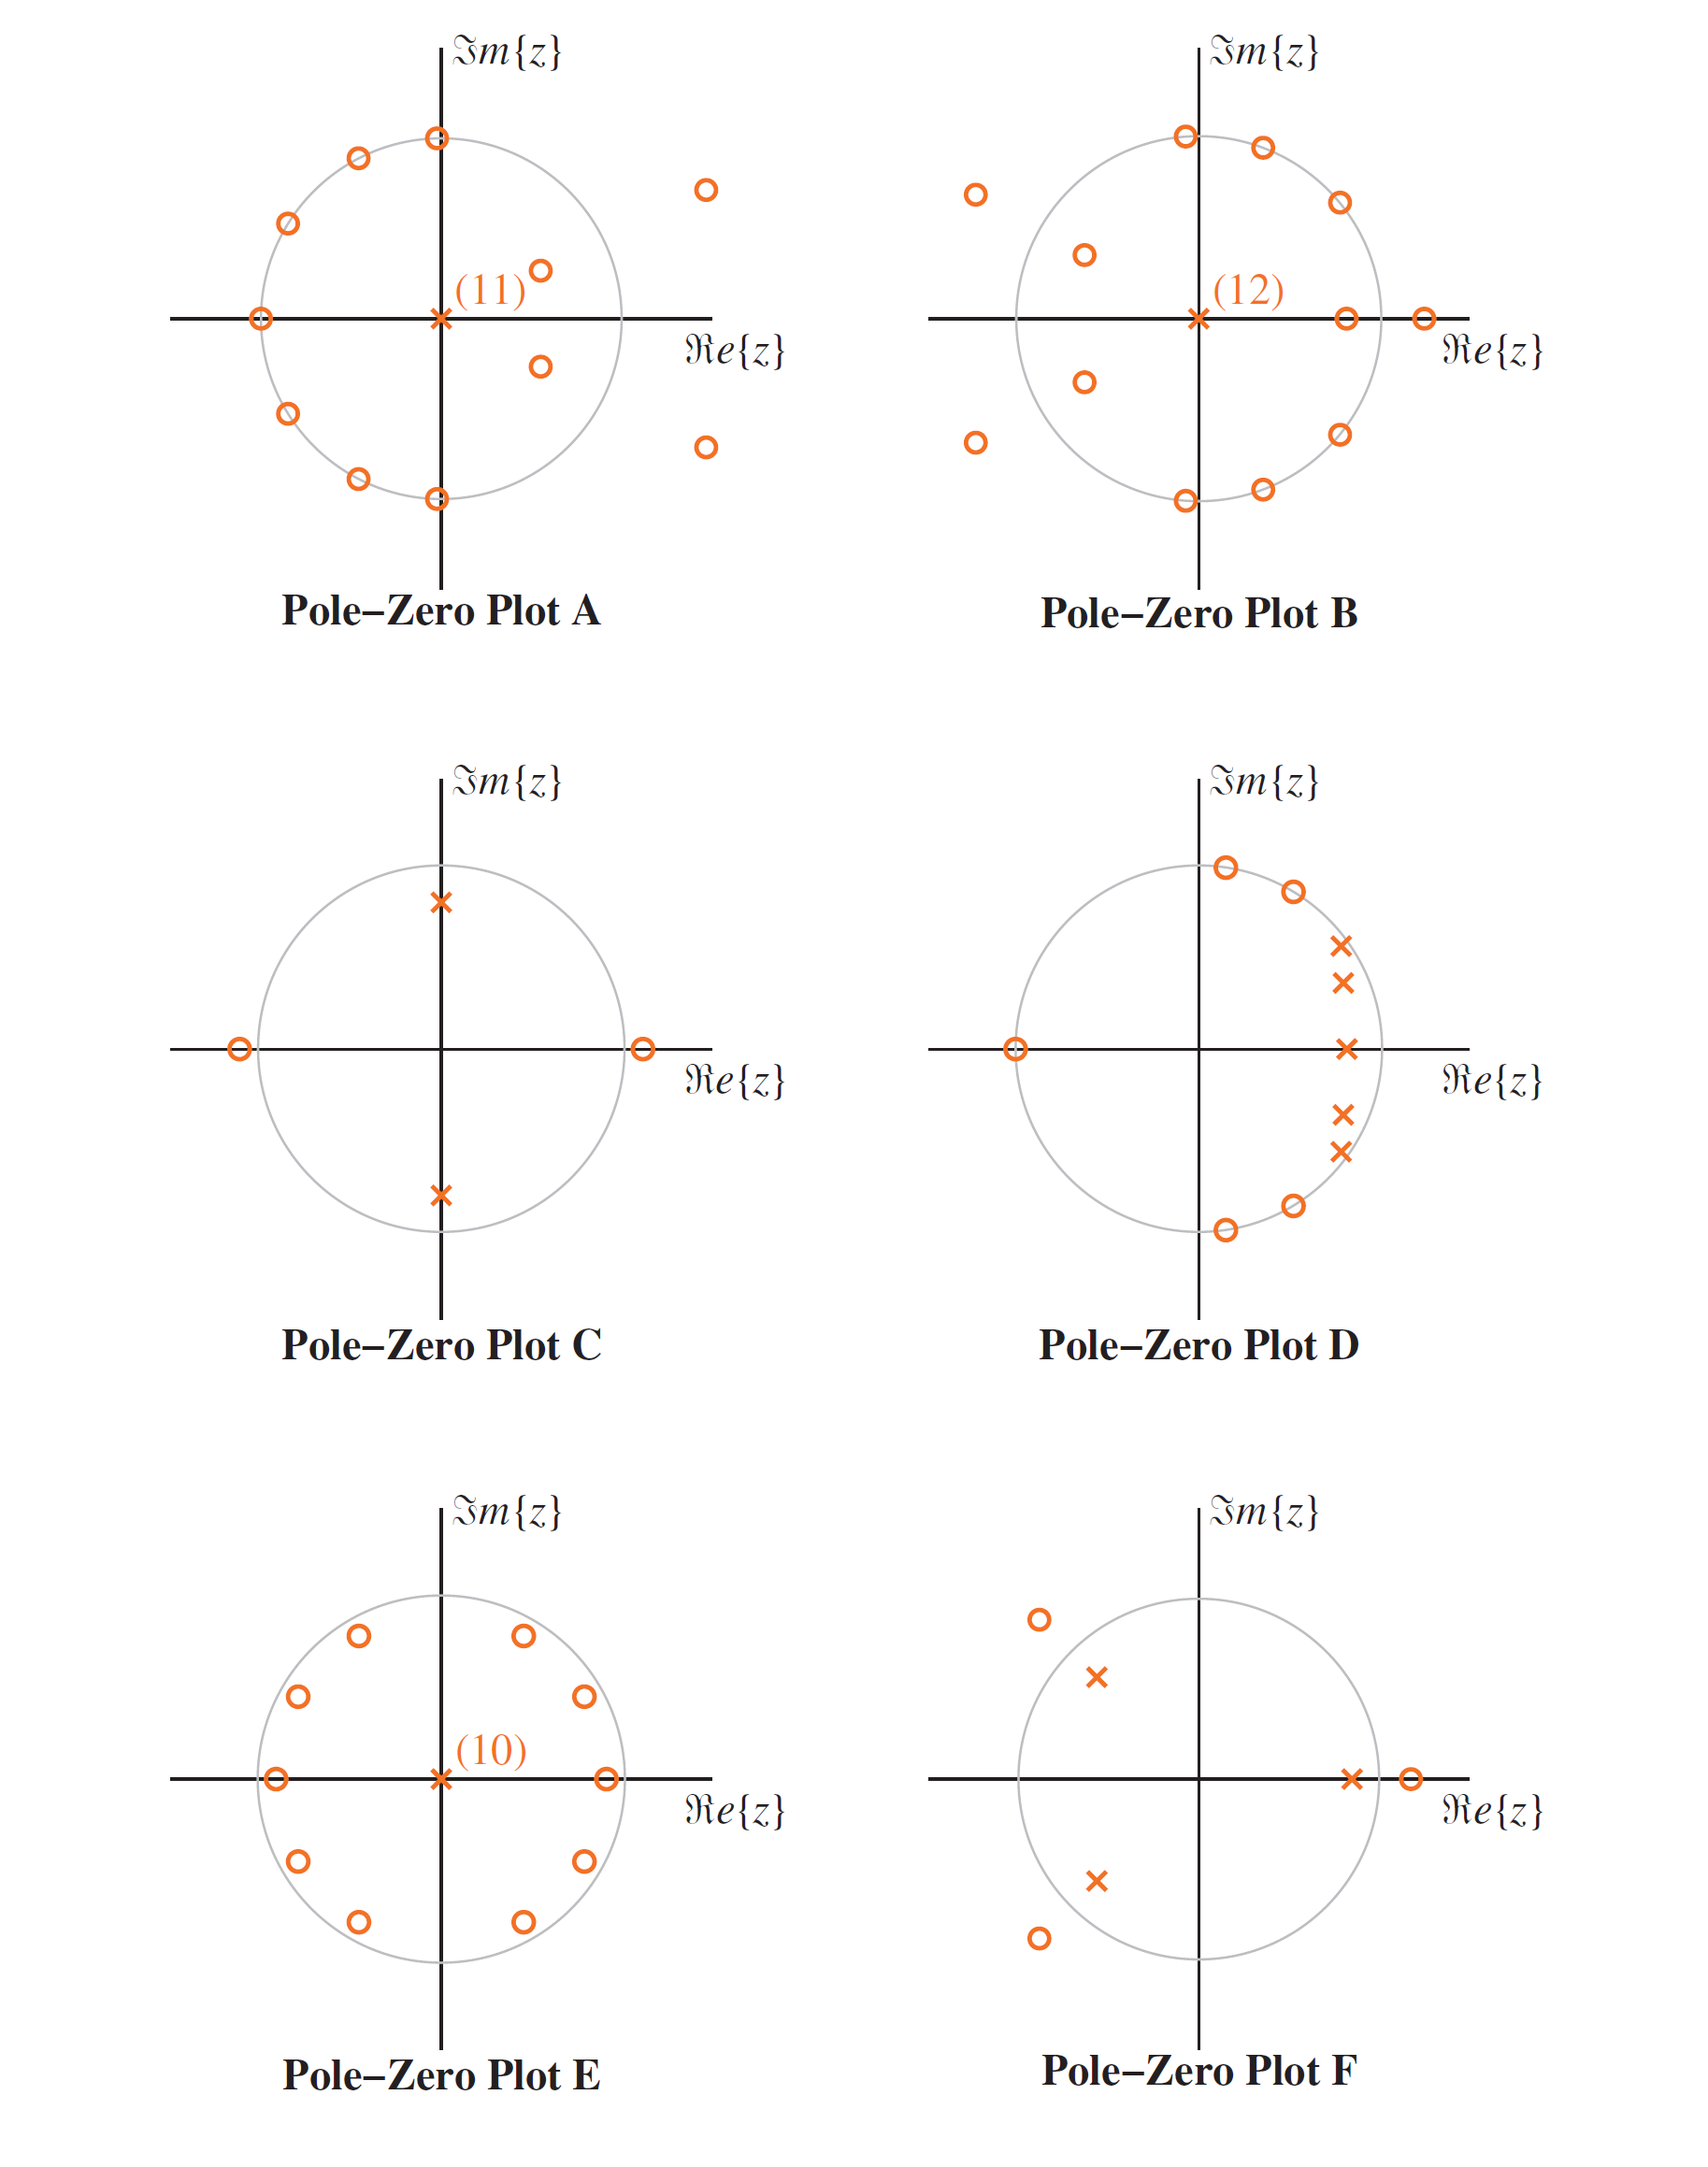
\includegraphics[scale=0.4]{figs/several_pole_zero_diagram.png}
	\caption{Pole-zero diagrams for problem 3. These diagrams describe six different \textbf{\underline{causal}} LTI systems; unit circle is shown for reference.}
	\label{fig:pole-zero-diagram}
\end{figure}


\newpage

\noindent {\bf Problem 4: Kramers-Kronig relations in discrete time (25 points)}

This problem will guide you through the proof of the Kramers-Kronig relations for \underline{discrete-time} signals, which establish that the real and imaginary parts of the DTFT of a \underline{real} and \underline{causal} signal $x[n] \Longleftrightarrow X(e^{j\omega}) = \mathrm{Re}\{X(e^{j\omega})\} + j\mathrm{Im}\{X(e^{j\omega})\}$ are related by 

\begin{align} \nonumber
\mathrm{Im}\{X(e^{j\omega})\} &= -\frac{1}{2\pi}\bigg[\Big(\frac{\sin\omega}{1-\cos\omega}\Big)\ast \mathrm{Re}\{X(e^{j\omega})\}\bigg] \\
&=-\frac{1}{2\pi}\int_{-\pi}^{\pi}\bigg(\frac{\sin\theta}{1-\cos\theta}\bigg)\mathrm{Re}\{X(e^{j(\omega-\theta)})\}d\theta
\end{align}

\noindent\textbf{Note:} This result looks a bit different from the one discussed in class, as in this problem you're working in discrete time. However, the same steps  can be followed to arrive at the result for continuous time. The only difference would be that in continuous time: $\mathcal{F}\{\mathrm{sign(t)}\} = -\frac{2j}{\Omega}, \Omega\neq 0$. Then, we would have
\begin{equation}
\mathrm{Im}\{X(j\Omega)\} = -\frac{1}{\pi\Omega}\ast \mathrm{Re}\{X(j\Omega)\} = -\mathcal{H}\{\mathrm{Re}\{X(j\Omega)\}\},
\end{equation}	
where this convolution is known as the Hilbert transform.


\begin{description}
	\item[(a)] \textbf{Even/odd decomposition}. Recall from lecture notes 1 that any signal $x[n] \leftrightarrow X(e^{j\omega})$ can be written as
	\begin{equation}
	x[n] = x_e[n] + x_o[n],
	\end{equation}
	where 
	\begin{align}
	x_e[n] = \frac{1}{2}(x[n] + x[-n]) \tag{even symmetric: $x_e[n] = x_e[-n]$} \\
	x_o[n] = \frac{1}{2}(x[n] - x[-n]) \tag{odd symmetric: $x_o[n] = -x_o[-n]$}
	\end{align}
	
	Assume that $x[n]$ is \underline{real} and write expressions for the DTFT of $x_e[n]$ and $x_o[n]$ as a function of $X(e^{j\omega})$.
	
	\textit{Hint:} Table 2.2 of the textbook lists useful properties of the DTFT.
	
	\item[(b)] Now assume that $x[n]$ is also \underline{causal} i.e., $x[n] = 0, n < 0$. Write an equation for $x_o[n]$ in terms of $x_e[n]$ only. Use this result to write an equation for $X_o(e^{j\omega}) = \mathcal{F}\{x_o[n]\}$ as a function of $X_e(e^{j\omega})=\mathcal{F}\{x_e[n]\}$ only.
	
	\textit{Hint:} You may use the following result:
	\begin{equation}
	\mathcal{F}\{\mathrm{sign[n]}\} = \begin{cases}
	-j\displaystyle\frac{\sin\omega}{1-\cos\omega}, &\omega\neq 0 \\
	0, &\omega = 0
	\end{cases}
	\end{equation} 
	
	\item[(c)] Combine your results of parts (a) and (b) to show that 
	
	\begin{equation}
	\mathrm{Im}\{X(e^{j\omega})\} = -\frac{1}{2\pi}\bigg[\Big(\frac{\sin\omega}{1-\cos\omega}\Big)\ast \mathrm{Re}\{X(e^{j\omega})\}\bigg]
	\end{equation}
\end{description} 


\mbox{}\\
\noindent {\bf Problem 5: ``Unknown'' plant identification by noise injection (35 points)} 

This problem deals with the plant identification by noise injection discussed on lecture notes 6, page 43. 

\begin{center}
	\resizebox{0.4\linewidth}{!}{\SimpleSys{../lectures/figs/simple_in_dsp_out}{$x[n]$}{$H(z) = ??$}{$y[n]$}}
\end{center}


To see how well that works, we'll assume that our plant is known and it is a \underline{lowpass} filter given by the following $z$-transform:
\begin{equation}
H(z) = 0.05634\frac{(1-0.9z^{-1})(1 -1.0166z^{-1} + 0.8z^{-2})}{(1-0.683z^{-1})(1 -1.4461z^{-1} + 0.7957z^{-2})}
\end{equation}

This system is minimum phase, as all its zeros are inside the unit circle. This system is already implemented for you on the file \texttt{plant\_id\_template.m}, available on Canvas (Files/Matlab).

\begin{description}
	\item[(a)] Plot the empirical autocorrelation function of the output of the plant $y[n]$ when the input is a white noise signal $x[n]$ with average power $\sigma_x^2 = 1$. 
	
	\textit{Hint:} you may use the Matlab functions \texttt{rand} or \texttt{randn} to generate the random signal. The distribution of the noise is not critical for this problem. To get accurate results generate a random vector with at least 50000 samples and use \texttt{maxLag = 256} in \texttt{xcorr}.
	
	\item[(b)] Use the function \texttt{[Phi, w] = calc\_psd(phi)} available on Canvas (Files/Matlab/) to obtain the empirical PSD and compare it with the theoretical PSD by plotting the empirical and theoretical PSDs on the same plot.
	
	\textit{Hint:} By calling \texttt{[H, w] = freqz(b, a, w)}, \texttt{freqz} will return the frequency response vector \texttt{H} evaluated at the frequencies \texttt{w}.
	
	\textbf{Note:} the function \texttt{[Phi, w] = calc\_psd(phi)} is simply using the FFT algorithm to calculate the DTFT of the autocorrelation function \texttt{phi} at the frequencies \texttt{w}. You'll learn how to use the FFT on lecture 11. This method of estimating the PSD is \underline{not} particularly good, as it requires too much data. On lecture 12, you'll  learn better ways of estimating the PSD.
		
	\item[(c)] Explain how you can use the results you proved in problem 4 to obtain the phase response. You may use the same strategy show in lecture notes 6, slide 41, but adapting it to discrete time.
	
	\item[(d)] Implement your method of part (c) and compare the estimated phase response with the true phase response of $H(z)$ by plotting them on the same plot. 
		
	\textit{Matlab hints:}
	\begin{itemize}
		\item In your method you will need to perform a convolution integral. You can still use the \texttt{conv} command for that. For instance,
		\begin{equation}
		\frac{1}{2\pi}\int_{-\pi}^{\pi}x(u)y(\omega-u)du \approx \texttt{1/(2*pi)*conv(x, y, `same')*dw},
		\end{equation}
		where the vectors $\texttt{x}$ and  $\texttt{y}$ are defined for $\texttt{w}$ between $[-\pi, \pi]$ in steps of $\texttt{dw}$. The parameter \texttt{`same'} just guarantees that the output vector will have the same length as \texttt{x} and \texttt{y}. This numerical integration method is equivalent to the trapezoidal rule.
		\item If your frequency vector \texttt{w} contains the zero frequency, you may want to enforce $\frac{\sin\omega}{1-\cos\omega}  = 0$ to prevent Matlab from generating a \texttt{NaN}.
	\end{itemize}
		
	\item[(e)] You should see that the phase response disagrees with the theoretical phase response for frequencies $|\omega| > \sim 0.3\pi$. Explain why there is a disagreement and whether this would be a problem in modeling that particular plant. 
\end{description}

\mbox{}\\
\rule{6.5 in}{0.5pt}
\textbf{Important:} The following problems correspond to lecture notes 7 and 8, which will be covered next Tuesday, July 25.

\mbox{}\\
\noindent {\bf Problem 6: (25 points)}

Consider the system of Example 5.8 of the textbook. Its system function is
\begin{equation}
H(z) = 0.05634\frac{(1+z^{-1})(1 -1.0166z^{-1} + z^{-2})}{(1-0.683z^{-1})(1 -1.4461z^{-1} + 0.7957z^{-2})}
\end{equation}

\begin{description}
	\item[(a)] Draw the signal flow graph of an implementation of the system as a cascade of a second-order system with a first-order system. Mark the values of the coefficients on the signal flow graph.
	\item[(b)] Draw a direct form II signal flow graph for implementing the system as a single third-order flow graph. 
	\item[(c)] Plot the pole-zero diagram of $H(z)$ for the unquantified coefficients. You may use \texttt{conv} to multiply out the numerator and denominator and obtain the coefficients vectors \texttt{a} and \texttt{b}. Then use \texttt{zplane} to plot the pole-zero diagram.
	\item[(d)] Quantize the filter coefficients with 6 bits to the right of the imagined binary point. Call the Q6-quantized coefficient vectors \texttt{ah} and \texttt{bh}. Then compare the pole-zero locations using
	\begin{align*}
		&\texttt{plot(roots(b),`ok');~plot(roots(a),`xk'); hold on} \\
		&\texttt{plot(roots(bh),`or');~plot(roots(ah),`xr');}
	\end{align*}
	
	Also plot the log magnitude of the frequency response of both the ``unquantized" and Q6-quantized coefficients on the same graph. Hand in both plots. You should observe that there is very little difference between the quantized and unquantized systems. What is your intuition about why this is so?
	
\end{description}

\mbox{}\\
\noindent {\bf Problem 7: (25 points)} (from the midterm of Spring-2014)

The following flow graphs represent equivalent difference equations for implementing a digital \underline{all-pass filter}. We will compare these systems when implemented with 16-bit fixed-point arithmetic. In the following diagrams, the signal values and constant multipliers are all scaled as $Q_{15}$ integers. The multiplications shown are quantized to 16 bits (15 bits plus a sign bit) \underline{directly after} the multiplication and \underline{before} any additions are done. Answer the questions below about the flow graphs.

\begin{center}
	\resizebox{0.5\textwidth}{!}{
\begin{tikzpicture}[node distance=1.75cm]
\node[terminal={below}{$x[n]$}] (x) at (0,0) {};
\node[terminal={below}{}, right of=x] (00) {};
\node[terminal={below}{}, right of= 00] (01) {};
\node[terminal={below}{}, right of=01] (02) {};
\node[terminal={below}{$y[n]$}, right of=02] (y) {};

\coordinate[below of=00] (10) {};
\node[terminal={below}{}, below of=01] (11) {};
\coordinate[below of=02] (12) {};

%
\draw[zpath={right}] (11) to (01);

%
\draw[solid, \thickness] (00) to (10);
\draw[solid, \thickness] (02) to (12);
%

%
\draw[amark={$-a$}{above}] (00) to (01);
\draw[amark={$1$}{above}] (10) to (11);

%
\draw[amark={$1$}{above}] (01) to (02);
\draw[amark={$a$}{above}] (12) to (11);

\draw[amark] (x) to (00);
\draw[amark] (02) to (y);
\node[black, fill=black!10, below=1.5cm of y] {(A)}; 
\end{tikzpicture}
}

\resizebox{0.5\textwidth}{!}{
\begin{tikzpicture}[node distance=1.75cm]
\node[terminal={below}{$x[n]$}] (x) at (0,0) {};
\node[terminal={below}{}, right=1cm of x] (00) {};
\node[terminal={below}{}, right=1.25cm of 00] (01) {};
\node[terminal={below}{}, right=1cm of 01] (02) {};
\node[terminal={below}{}, right=1.25cm of 02] (03) {};
\node[terminal={below}{$y[n]$}, right=1cm of 03] (y) {};

\node[terminal={below}{}, below of=00] (10) {};
\coordinate[below of=01] (11) {};
\coordinate[below of=02] (12) {};
\node[terminal={below}{}, below of=03] (13) {};

%
\draw[zpath={left}] (00) to (10);
\draw[amark={$1$}{below}] (10) to (11);
\draw[solid, \thickness] (11) to (01);

%
\draw[zpath={right}] (03) to (13);
\draw[amark={$a$}{below}] (13) to (12);
\draw[solid, \thickness] (12) to (02);

%
\draw[amark={}{right}] (x) to (00);
\draw[amark={$-a$}{above}] (00) to (01);
\draw[amark={}{right}] (01) to (02);
\draw[amark={}{right}] (03) to (y);

\draw[amark={$1$}{above}] (02) to (03);


\node[black, fill=black!10, below=1.5cm of y] {(B)}; 
\end{tikzpicture}
}

\resizebox{0.5\textwidth}{!}{
	\begin{tikzpicture}[node distance=1.75cm]
	\node[terminal={below}{$x[n]$}] (x) at (0,0) {};
	\node[terminal={below}{}, right of=x] (00) {};
	\node[terminal={below}{}, right of= 00] (01) {};
	\node[terminal={below}{}, right of=01] (02) {};
	\node[terminal={below}{$y[n]$}, right of=02] (y) {};
	
	\coordinate[below of=00] (10) {};
	\node[terminal={below}{}, below of=01] (11) {};
	\coordinate[below of=02] (12) {};
	
	%
	\draw[amark={$a$}{right}] (11) to (01);
	
	%
	\draw[solid, \thickness] (00) to (10);
	\draw[solid, \thickness] (02) to (12);
	%
	
	%
	\draw[amark={$z^{-1}$}{above}] (00) to (01);
	\draw[amark={$-1$}{above}] (10) to (11);
	
	%
	\draw[amark={$1$}{above}] (01) to (02);
	\draw[amark={$z^{-1}$}{above}] (12) to (11);
	
	\draw[amark] (x) to (00);
	\draw[amark] (02) to (y);
	\node[black, fill=black!10, below=1.5cm of y] {(C)}; 
	\end{tikzpicture}
}

\resizebox{0.5\textwidth}{!}{
	\begin{tikzpicture}[node distance=1.75cm]
	\node[terminal={below}{$x[n]$}] (x) at (0,0) {};
	\node[terminal={below}{}, right of=x] (00) {};
	\node[terminal={below}{}, right of= 00] (01) {};
	\node[terminal={below}{}, right of=01] (02) {};
	\node[terminal={below}{$y[n]$}, right of=02] (y) {};
	
	\coordinate[below of=00] (10) {};
	\node[terminal={below}{}, below of=01] (11) {};
	\coordinate[below of=02] (12) {};
	
	%
	\draw[amark={$z^{-1}$}{right}] (01) to (11);
	
	%
	\draw[solid, \thickness] (00) to (10);
	\draw[solid, \thickness] (02) to (12);
	%
	
	%
	\draw[amark={$1$}{above}] (00) to (01);
	\draw[amark={$a$}{above}] (11) to (10);
	
	%
	\draw[amark={$-a$}{above}] (01) to (02);
	\draw[amark={$1$}{above}] (11) to (12);
	
	\draw[amark] (x) to (00);
	\draw[amark] (02) to (y);
	\node[black, fill=black!10, below=1.5cm of y] {(D)}; 
	\end{tikzpicture}
}
\end{center}

\begin{description}
	\item[(a)] What is the system $H(z)$ that describes all the above systems when the difference equations are implemented without quantization?
	\item[(b)] Re-draw the signal plow graphs inserting noise sources to represent quantization of the multiplications. Mark each of them with the symbol $\sigma_{15}^2$ denoting the average power of the source. Give a formula for $\sigma_{15}^2$.
	\item[(c)] Assuming that $|a|<1$, and that the output of each system is represented as $\hat{y}[n] = y[n] + f[n]$, determine the power spectrum, $\Phi_{ff}(e^{j\omega})$, of the noise component, $f[n]$, for each flow graph. Be sure to combine independent noise sources to simplify the analysis.
	\item[(d)] For which system will the total noise power be the largest? Determine a closed-form formula for the largest total noise power, $\sigma_f^2$. Your equations should be a function of $\sigma_{15}^2$ and $a$ only.
	
\textit{Hint:} When calculating the total noise power, please avoid the frequency domain integration.
\end{description}

\newpage
\noindent \textbf{Attachment}\\
\rule{6.5 in}{0.5pt}

\begin{figure}[h!]
	\centering
	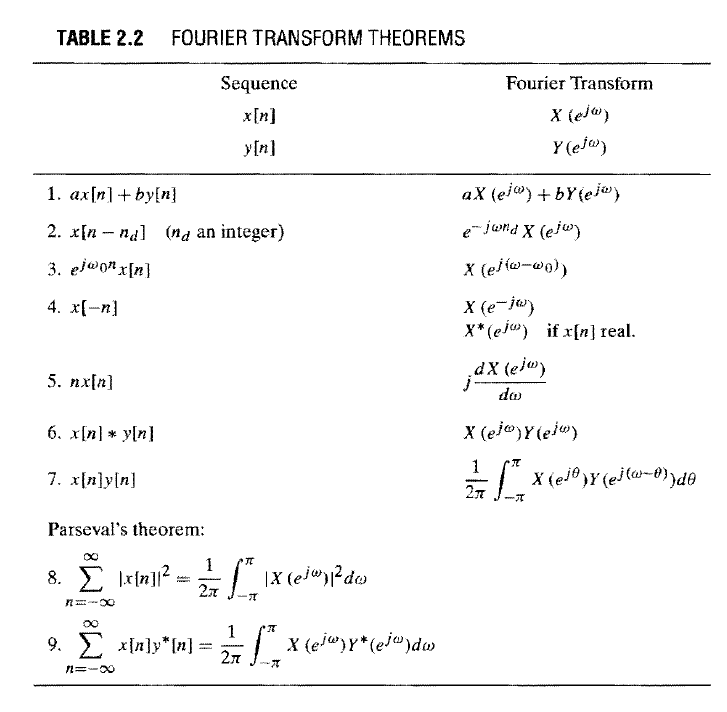
\includegraphics{figs/table22.png}
	\caption{Table 2.2 of the textbook.}
\end{figure}

\end{document}
